\begin{center}
\chapter{An\'alisis}
\end{center}
\newpage

\section{Sistema operativo y platadorma de desarrollo}
EL cuadro \ref{tab:t21} es la comparativa de las plataformas que se analizaron para la elaboración del trabajo terminal.

\begin{table}[H]
\centering
\resizebox{\textwidth}{!}{%
\begin{tabular}{
>{\columncolor[HTML]{C0C0C0}}l lll}
\hline
\multicolumn{4}{c}{\cellcolor[HTML]{9B9B9B}{\color[HTML]{333333} \textbf{Plataforma Windows}}} \\
\multicolumn{1}{c}{\cellcolor[HTML]{9B9B9B}{\color[HTML]{333333} \textbf{Descripción}}} &
  \multicolumn{1}{c}{\cellcolor[HTML]{9B9B9B}{\color[HTML]{333333} \textbf{Software}}} &
  \multicolumn{1}{c}{\cellcolor[HTML]{9B9B9B}{\color[HTML]{333333} \textbf{Costo}}} &
  \multicolumn{1}{c}{\cellcolor[HTML]{9B9B9B}{\color[HTML]{333333} \textbf{Operatividad}}} \\
Sistema Operativo &
  Windows 10 Pro &
  MXN\$5,199.00 &
  \begin{tabular}[c]{@{}l@{}}Ideal para pequeñas empresas o\\  usuarios que necesiten una\\  funcionalidad mejorada.\end{tabular} \\
Sistema Operativo &
  Windows 10 Home &
  MXN\$3,599.00 &
  Ideal para uso personal o doméstico. \\
Sistema Operativo &
  Windows 10 Pro para Workstations &
  MXN\$7,899.00 &
  \begin{tabular}[c]{@{}l@{}}Ideal para los usuarios avanzados y\\  pequeñas empresas que buscan \\ funcionalidad mejorada con la \\ capacidad de calcular cargas de\\  trabajo intensivas.\end{tabular} \\
Sistema Operativo &
  Windows Server 2019 &
  MXN\$10,814.69 &
  \begin{tabular}[c]{@{}l@{}}Sistema operativo que une los entornos\\  on-premises con Azure y agrega capas\\  adicionales de seguridad a la vez que\\  te ayuda a modernizar tus aplicaciones\\  e infraestructura.\end{tabular}
\end{tabular}%
}
\caption{Sistemas operativos de plataforma Windows}
\label{tab:t21}
\end{table}

El cuadro \ref{tab:t22} muestra la comparativa de las plataformas de desarrollo que se analizaron para la elaboración del trabajo terminal.

\begin{table}[H]
\resizebox{\textwidth}{!}{%
\begin{tabular}{|c|c|c|l|}
\hline
\rowcolor[HTML]{9B9B9B} 
\multicolumn{4}{|c|}{\cellcolor[HTML]{9B9B9B}\textbf{Plataforma de desarrollo}}                                                \\ \hline
\rowcolor[HTML]{9B9B9B} 
\textbf{Descripción} & \textbf{Software} & \textbf{Costo} & \multicolumn{1}{c|}{\cellcolor[HTML]{9B9B9B}\textbf{Operatividad}} \\ \hline
\cellcolor[HTML]{C0C0C0}Motor de Desarrollo &
  Unity Free &
  Gratis &
  \begin{tabular}[c]{@{}l@{}}Unity es un motor de videojuego\\  multiplataforma creado por Unity Technologies.\\  Unity está disponible como plataforma de desarrollo\\  para Microsoft Windows, Mac OS, Linux. \\ La plataforma de desarrollo tiene soporte de compilación\\  con diferentes tipos de plataformas\end{tabular} \\ \hline
\cellcolor[HTML]{C0C0C0}Motor de Desarrollo &
  Unreal Engine 4 &
  Gratis &
  \begin{tabular}[c]{@{}l@{}}Unreal Engine es un motor de juego creado por la compañía\\  Epic Games, mostrado inicialmente en el shooter en primera\\  persona Unreal en 1998. \\ Aunque se desarrolló principalmente para los shooters en primera\\  persona, se ha utilizado con éxito en una variedad de otros géneros.\end{tabular} \\ \hline
\end{tabular}%
}
\caption{Plataforma de desarrollo.
}
\label{tab:t22}
\end{table}

Tomando en cuenta la infraestructura que posee la Escuela Superior de Medicina del Instituto Politécnico Nacional, específicamente el Departamento de Computación se optó por usar el sistema operativo Windows 10 Pro y Unity ®.

\section{Hardware}
De acuerdo a las especificaciones del software seleccionado se recomienda usar:\\
\begin{itemize}
\item Tarjeta Gráfica: NVIDIA GTX 1060 / AMD Radeon RX 480 o mejor
\item Tarjeta Gráfica Alternativa: NVIDIA GTX 970 / AMD Radeon R9 290 o mejot
\item CPU: Intel i5-4590 / AMD Ryzen 5 1500X o mejor
\item Memoria: 8GB+ RAM
\item Salida de Video: Compatible HDMI 1.3 video output
\item USB puertos: 3x USB 3.0 y  1x USB 2.0
\end{itemize}
Y en caso de no contar con estos elementos, el mínimo es:
\begin{itemize}
\item Tarjeta Gráfica: NVIDIA GTX 1050Ti / AMD Radeon RX 470 o mejor
\item Tarjeta Gráfica Alternativa: NVIDIA GTX 960 / AMD Radeon R9 290 o mejor
\item CPU: Intel i3-6100 / AMD Ryzen 3 1200, FX4350 o mejor
\item Memoria: 8GB+ RAM
\item Salida de Video: Compatible HDMI 1.3 video output
\item Puertos USB: 1x USB 3.0 y 2x USB 2.0
\end{itemize} 

\section{Viabilidad}
También se analizó la factibilidad del proyecto en general. Desde el punto de vista técnico se realizó una evaluación de la tecnología actual existente y la posibilidad de utilizarla en el desarrollo del sistema. Además de DirectX versión 11 el cuadro \ref{tab:t23} muestra los recursos técnicos necesarios para la ejecución correcta del software:\\
\begin{table}[H]
\centering
\begin{tabular}{|c|c|l|}
\hline
\rowcolor[HTML]{9B9B9B} 
\textbf{Cantidad} &
  \textbf{Recursos} &
  \multicolumn{1}{c|}{\cellcolor[HTML]{9B9B9B}\textbf{Características}} \\ \hline
\cellcolor[HTML]{C0C0C0}1 &
  Computadora Personal de Escritorio &
  \begin{tabular}[c]{@{}l@{}}Tarjeta gráfica discreta, RX480\\ Memoria RAM 16 Gb\\ 5 Puertos USB\\ Procesador de 4 núcleos o mayor\end{tabular} \\ \hline
\cellcolor[HTML]{C0C0C0}1 &
  Sistema de realidad Virtual Oculus Rift &
  \begin{tabular}[c]{@{}l@{}}Visor HMD, controles Touch \\ \\ Sensores Touch.\end{tabular} \\ \hline
\end{tabular}
\caption{ Recursos Técnicos.}
\label{tab:t23}
\end{table}
Económicamente, se determinaron los recursos para desarrollar el sistema así como la comparativa con el uso de cuerpos para su examinación y estudio. Después de un análisis e investigación de los costos con la dirección del Área de Morfología en la Escuela Superior de Medicina bajo la asesoría del Dr. Macias Rios se determinó que el costo que se tiene para el traslado, mantenimiento, uso e inhumación de los cuerpos es de \$40,000.00 c/u, como se ve en el cuadro \ref{tab:t24}.
\begin{table}[H]
\centering
\begin{tabular}{|
>{\columncolor[HTML]{C0C0C0}}c |l|}
\hline
\multicolumn{2}{|c|}{\cellcolor[HTML]{9B9B9B}\textbf{Costo de uso de cuerpos.}} \\ \hline
Traslado, mantenimiento, uso e inhumación           & \$40,000.00 c/u           \\ \hline
Total                                               & \$40,000.00 c/u           \\ \hline
\end{tabular}
\caption{Costo de cálculo de uso de cuerpos.}
\label{tab:t24}
\end{table}

En el caso del desarrollo e implementación del proyecto se consideró la depreciación, como se observa en el cuadro \ref{tab:t25}.
\begin{table}[H]
\centering
\resizebox{\textwidth}{!}{%
\begin{tabular}{clccccc|c|c|}
\hline
\rowcolor[HTML]{9B9B9B} 
\multicolumn{9}{|c|}{\cellcolor[HTML]{9B9B9B}\textbf{Depreciaciones del Proyecto}} \\ \hline
\rowcolor[HTML]{9B9B9B} 
\multicolumn{4}{|c|}{\cellcolor[HTML]{9B9B9B}\textbf{Equipos de Cómputo}} &
  \multicolumn{5}{c|}{\cellcolor[HTML]{9B9B9B}\textbf{Depreciación}} \\ \hline
\rowcolor[HTML]{9B9B9B} 
\multicolumn{1}{|c|}{\cellcolor[HTML]{9B9B9B}\textbf{Cantidad}} &
  \multicolumn{1}{c|}{\cellcolor[HTML]{9B9B9B}\textbf{Equipos}} &
  \multicolumn{1}{c|}{\cellcolor[HTML]{9B9B9B}\textbf{\begin{tabular}[c]{@{}c@{}}Monto original de \\ Inversión\end{tabular}}} &
  \multicolumn{1}{c|}{\cellcolor[HTML]{9B9B9B}\textbf{\begin{tabular}[c]{@{}c@{}}Valor actual\\  del equipo\end{tabular}}} &
  \multicolumn{1}{c|}{\cellcolor[HTML]{9B9B9B}\textbf{\begin{tabular}[c]{@{}c@{}}Valor a \\ \\ depreciar\end{tabular}}} &
  \multicolumn{1}{c|}{\cellcolor[HTML]{9B9B9B}\textbf{\begin{tabular}[c]{@{}c@{}}\%\\ anual\end{tabular}}} &
  \textbf{\begin{tabular}[c]{@{}c@{}}\%\\ mensual\end{tabular}} &
  \textbf{\begin{tabular}[c]{@{}c@{}}Depresiación\\ mensual\end{tabular}} &
  \textbf{\begin{tabular}[c]{@{}c@{}}Depreciación\\ anual\end{tabular}} \\ \hline
\multicolumn{1}{|c|}{\cellcolor[HTML]{C0C0C0}1} &
  \multicolumn{1}{l|}{\begin{tabular}[c]{@{}l@{}}Computadora de\\ escritorio armada\end{tabular}} &
  \multicolumn{1}{c|}{\$25,054.63} &
  \multicolumn{1}{c|}{\$20,000.00} &
  \multicolumn{1}{c|}{\$5,054.63} &
  \multicolumn{1}{c|}{33.33\%} &
  2.78\% &
  \$ 140.52 &
  \$1,545.72 \\ \hline
\multicolumn{1}{|c|}{\cellcolor[HTML]{C0C0C0}1} &
  \multicolumn{1}{l|}{Laptop HP} &
  \multicolumn{1}{c|}{\$9,999.00} &
  \multicolumn{1}{c|}{\$6,999.00} &
  \multicolumn{1}{c|}{\$3,000.00} &
  \multicolumn{1}{c|}{33.33\%} &
  2.78\% &
  \$ 83.40 &
  \$ 917.40 \\ \hline
\multicolumn{7}{l}{} &
  \textbf{Total:} &
  \$ 2,463.12 \\ \cline{8-9} 
\end{tabular}
}
\caption{Depreciaciones del proyecto.}
\label{tab:t25}
\end{table}

Para ofrecer una experiencia aceptable al momento del uso del equipo de Realidad Virtual y el software se proponen los elementos del cuadro \ref{tab:t26}.
%%
  %Tabla de costos de productos, no se ha logrado realizar correctamente%
%%
\textbf{Pendiente tabla costos}\\
Además, el sistema de Realidad Virtual con sus componentes tiene un costo que se muestra en el cuadro \ref{tab:t27}.
\begin{table}[H]
  \centering
  \begin{tabular}{|c|c|}
  \hline
  \rowcolor[HTML]{9B9B9B} 
  \multicolumn{2}{|c|}{\cellcolor[HTML]{9B9B9B}\textbf{Sistema de Realidad Virtual}} \\ \hline
  \rowcolor[HTML]{9B9B9B} 
  \textbf{Producto}                          & \textbf{Producto}                     \\ \hline
  Visor Oculus Rift                          & Incluido en el paquete                \\ \hline
  Controles Touch Oculus x 2                 & Incluido en el paquete                \\ \hline
  Sensores Oculus x 2                        & Incluido en el paquete                \\ \hline
  Anexos                                     & Incluido en el paquete                \\ \hline
  \textbf{Total:}                            & \$ 8,821.74                           \\ \hline
  \end{tabular}
  \caption{Costos y contenido del sistema de Realidad Virtual.}
  \label{tab:t27}
\end{table}

Se estimaron los suelos de programador y modelado, como se observa en la tabla \ref{tab:t28}.\\
\begin{table}[H]
  \centering
  \resizebox{\textwidth}{!}{%
  \begin{tabular}{ccc|c|c|}
  \hline
  \rowcolor[HTML]{9B9B9B} 
  \multicolumn{5}{|c|}{\cellcolor[HTML]{9B9B9B}\textbf{Sueldos}}                                                                                                                                                                                                                                                                    \\ \hline
  \rowcolor[HTML]{9B9B9B} 
  \multicolumn{1}{|c|}{\cellcolor[HTML]{9B9B9B}\textbf{Puesto}} & \multicolumn{1}{c|}{\cellcolor[HTML]{9B9B9B}\textbf{\begin{tabular}[c]{@{}c@{}}Sueldo\\ Mensual\\ individual\end{tabular}}} & \textbf{\begin{tabular}[c]{@{}c@{}}Cantidad \\ \\ de personal\end{tabular}} & \textbf{Sueldos mensuales totales} & \textbf{6 meses} \\ \hline
  \multicolumn{1}{|c|}{Programador}                             & \multicolumn{1}{c|}{\$25,296.00}                                                                                            & 1                                                                           & \$25,296.00                        & \$151,776.00     \\ \hline
  \multicolumn{1}{|c|}{Modelador 3D}                            & \multicolumn{1}{c|}{\$25,296.00}                                                                                            & 1                                                                           & \$25,296.00                        & \$151,776.00     \\ \hline
  \multicolumn{3}{l}{}                                                                                                                                                                                                                                                      & \multicolumn{1}{l|}{Total}         & \$303,522.00     \\ \cline{4-5} 
  \end{tabular}%
  }
  \caption{Cálculo de Sueldos.
  }
  \label{tab:t28}
\end{table}

\begin{table}[H]
  \centering
  \begin{tabular}{c|c|c|}
  \hline
  \rowcolor[HTML]{9B9B9B} 
  \multicolumn{3}{|c|}{\cellcolor[HTML]{9B9B9B}\textbf{Servicios}}                                       \\ \hline
  \rowcolor[HTML]{9B9B9B} 
  \multicolumn{1}{|c|}{\cellcolor[HTML]{9B9B9B}\textbf{Concepto}} & \textbf{Mensual} & \textbf{11 Meses} \\ \hline
  \multicolumn{1}{|c|}{Luz (kw Consumidos por costo Unitario)}    & \$430            & \$4,730           \\ \hline
  \multicolumn{1}{|c|}{Agua (Lt consumidos por costo unitario)}   & \$200            & \$2,200           \\ \hline
  \multicolumn{1}{|c|}{Teléfono e Internet (renta mensual fija)}  & \$ 450           & \$4,850           \\ \hline
  \multicolumn{1}{l|}{}                                           & Total:           & \$11,780          \\ \cline{2-3} 
  \end{tabular}
  
  \caption{Cálculo de Costo por Servicios.}
  \label{tab:t29}
\end{table}

Los servicios estimados se muestran en el cuadro \ref{tab:t29} y en el cuadro \ref{tab:t210} se muestra la suma total y como resultado se obtiene el costo total del proyecto, que se estima en: \$326,316.86.\\
\begin{table}[H]
  \centering
  \begin{tabular}{|l|r|}
  \hline
  \rowcolor[HTML]{9B9B9B} 
  \multicolumn{2}{|c|}{\cellcolor[HTML]{9B9B9B}\textbf{Costos del Proyecto}}                                                    \\ \hline
  \rowcolor[HTML]{9B9B9B} 
  \multicolumn{1}{|c|}{\cellcolor[HTML]{9B9B9B}\textbf{Concepto}} & \multicolumn{1}{c|}{\cellcolor[HTML]{9B9B9B}\textbf{Costo}} \\ \hline
  Servicios                                                       & \$ 11,780                                                   \\ \hline
  Sueldos                                                         & \$303,522.00                                                \\ \hline
  Depreciaciones                                                  & \$2,463.12                                                  \\ \hline
  Equipo extra.                                                   & \$ 8,821.74                                                 \\ \hline
  Total                                                           & \$ 326,316.86                                               \\ \hline
  \end{tabular}
  \caption{Costos finales del proyecto}
  \label{tab:my-t210}
  \end{table}

En resumen, el costo de usar nueve cuerpos sería de \$360,000.00 y el del proyecto de \$326,318.00, con lo cual se puede considerar viable económicamente.\\

\section{Análisis de la plataforma Unity ®}
Unity ® es un motor de desarrollo de videojuegos multiplataforma desarrollado por Unity ® Technologies. Con él se pueden crear videojuegos, simuladores, software de realidad virtual y aumentada. Puede generar código para computadoras de escritorio, portátiles, consolas de videojuegos, Smart TV y otros dispositivos móviles. Ofrece una API de scripting en C\#. En la figura 8 se puede ver el entorno en general.\\
\begin{figure}[H]
	\begin{center}
 		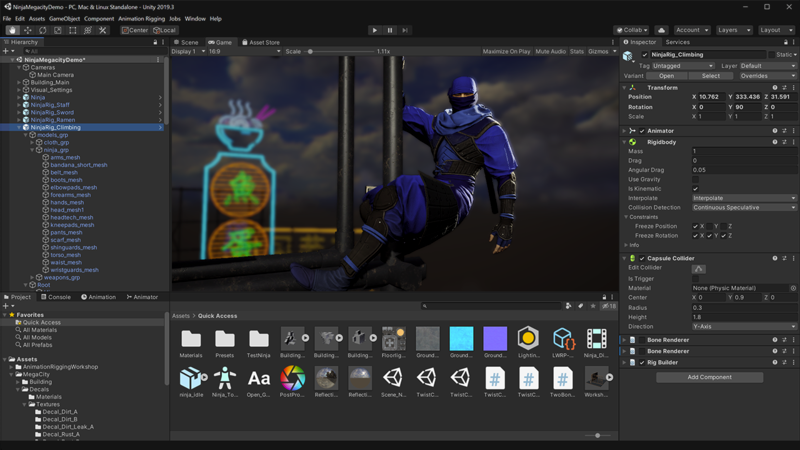
\includegraphics[width = .5\textwidth]{source/images/image33.png}
 		\captionof{figure}{\label{fig:im20}Interfaz de trabajo de Unity ®3D en 2020 \cite{wiki1}}
	\end{center} 
\end{figure}

\section{Sistema de Seguimiento}
Cada dispositivo rastreador tiene una "constelación" predefinida de LED infrarrojos ocultos debajo del plástico externo, que puede ver resaltado en la figura 9. La luz IR es invisible para el ojo humano.\\
\begin{figure}[H]
	\begin{center}
 		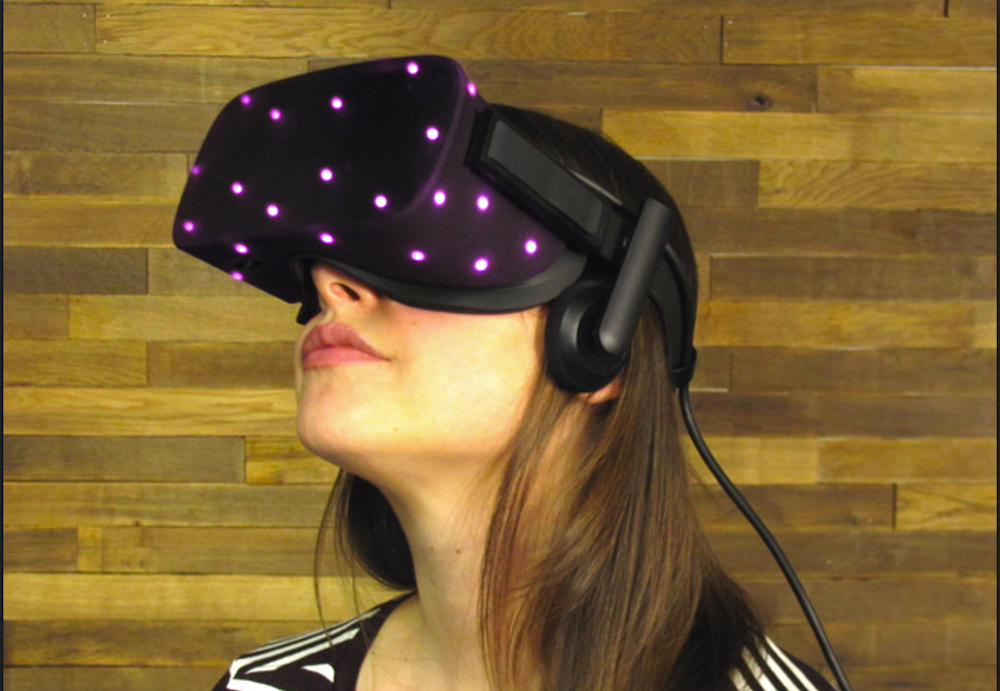
\includegraphics[width = .5\textwidth]{source/images/image55.png}
 		\captionof{figure}{\label{fig:im21}Muestra de el diseño de la “constelación” incluida en el Oculus Rift ®}
	\end{center} 
\end{figure}
Los sensores, que son esencialmente cámaras con filtros para ver sólo la luz IR, envían cuadros a la PC del usuario a través de un cable USB a 60 Hz. La PC procesa cada cuadro, identificando la posición de cada LED IR y, por lo tanto, la posición relativa de cada objeto.\\
El software puede reconocer fácilmente qué LED está viendo porque conoce la forma de la "constelación", recuerda dónde estaba el objeto en el cuadro anterior y conoce su dirección de aceleración (desde el acelerómetro) y su rotación (desde giroscopio). Cada LED IR también parpadea a una frecuencia específica para identificarse.\\
Estas innovaviones le provieron a "Constellation" de una ventaja sobre los sistemas de seguimiento anteriores.\\
\begin{figure}[H]
	\begin{center}
 		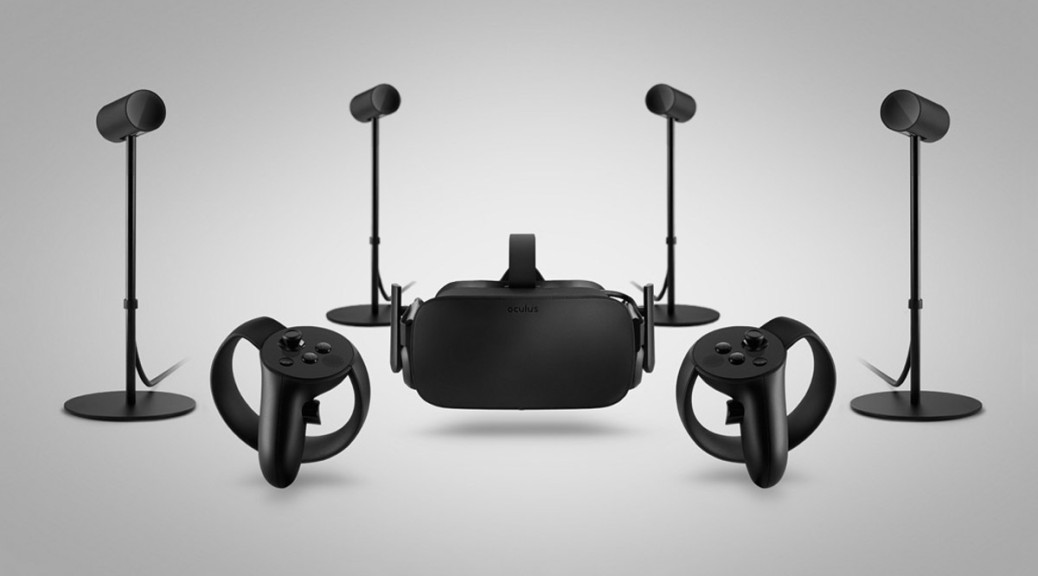
\includegraphics[width = .5\textwidth]{source/images/image15.png}
 		\captionof{figure}{\label{fig:im22}Visor Oculus Rift ®, controles Oculus Touch ® y sensores Oculus Sensor ®}
	\end{center} 
\end{figure}
Para admitir el movimiento rápido, los auriculares Rift y los controladores táctiles se comunican de forma inalámbrica con un chip inalámbrico en el sensor cada vez que están a punto de pulsar sus LED. Esto permite que el obturador de la cámara se dispare exactamente como lo hacen los LED, y permite que la exposición sea corta.\\

\section{Análisis de Información médica}
El cuerpo humano es una estructura compleja y altamente organizada, formada por células que trabajan juntas para realizar funciones específicas necesarias para mantener la vida.\cite{web10}.\\
La biología del cuerpo humano incluye:\\
\begin{itemize}
  \item Fisiología (cómo funciona el cuerpo)
  \item Anatomía (cómo se estructura el cuerpo)
  \end{itemize}
\begin{figure}[H]
	\begin{center}
 		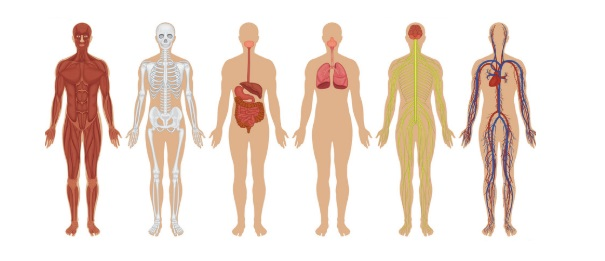
\includegraphics[width = .5\textwidth]{source/images/image22.png}
 		\captionof{figure}{\label{fig:im23}Gráfico ejemplificando los sistemas del cuerpo humano.\cite{web11}}
	\end{center} 
\end{figure}

\subsection{Cavidad abdominal}
Para el desarrollo del trabajo terminal interesa la cavidad abdominal, que es el espacio corporal que ocupa la región del abdomen, ubicada entre el diafragma y la abertura de la pelvis. Es la cavidad más grande del cuerpo humano y contiene los principales órganos del aparato digestivo, urinario y genital.\\
Para su estudio y evaluación clínica en el campo de la medicina, el abdomen debe ser dividido topográficamente de forma externa en 9 cuadrantes o regiones, utilizando cuatro líneas trazadas imaginariamente, dos verticales y dos horizontales.\cite{web12}\\
\begin{figure}[H]
	\begin{center}
 		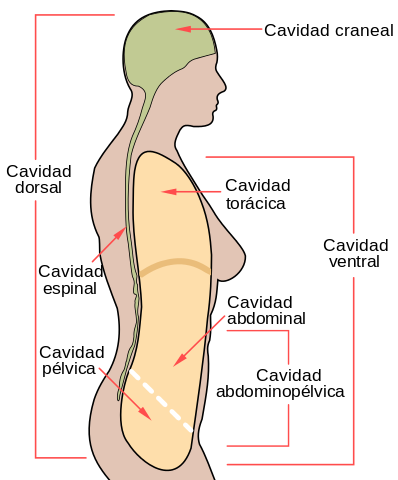
\includegraphics[width = .3\textwidth]{source/images/image56.png}
 		\captionof{figure}{\label{fig:im24}Diagrama que muestra las diferentes cavidades del cuerpo humano.}
	\end{center} 
\end{figure}
A continuación se muestra una representación del sistema digestivo, está contienen la información de cuáles son los órganos y elementos que lo conforman, estos serán varios ya que se han tomado como guía, estos elegidos mediante a una entrevista de estudiantes de medicina como material que se ha utilizado para el estudio del cuerpo humano, para la realización de modelos en 3D, asimismo, ejemplifica el material que dispone pero no limitado a el alumnado para el estudio del sistema en cuestión.\\
Aunado a esto se incorporan la mayoría de los elementos del sistema digestivo los cuales se encuentran en la cavidad abdominal estos expuestos por autores de los diferentes materiales en los cuales, pero no limitados a estos, se realizó la investigación del sistema.\\
\begin{figure}[H]
	\begin{center}
 		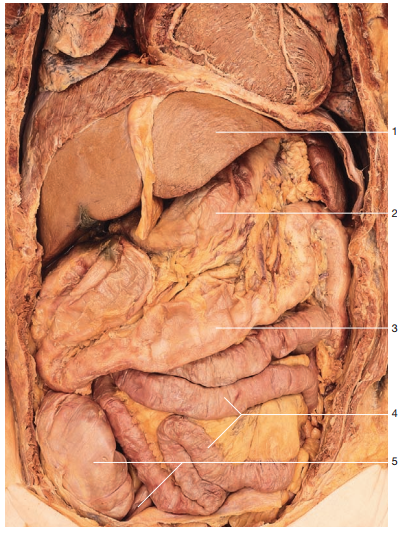
\includegraphics[width = .3\textwidth]{source/images/image72.png}
 		\captionof{figure}{\label{fig:im25}Órganos digestivos in situ (El epiplón mayor ha sido parcialmente eliminado o reflejado)\cite{rohen2018anatomy}}
	\end{center} 
\end{figure}
\begin{enumerate}
  \item Hígado
  \item Estómago
  \item Colon transverso
  \item Intestino delgado
  \item Ciego con apéndice vermiforme
\end{enumerate}
Para efectos de este Trabajo Terminal solamente se desarrolló el sistema digestivo, ubicado en la cavidad abdominal, para su interacción mediante realidad virtual con el mismo.\\
\subsection{Sistema Digestivo}
El tubo digestivo se compone de diferentes secciones: boca, esófago, estómago, intestino delgado, intestino grueso, recto y ano. Cada una de estas estructuras tiene elementos en común y algunos otros que las diferencian entre ellas.\cite{rouviere2005anatomia}\\ 
Cabe mencionar que el sistema digestivo también incluye órganos situados fuera del tubo digestivo los cuales son, el páncreas, el hígado y la vesícula biliar. Para los efectos del trabajo terminal el sistema digestivo será resumido en los elementos contenidos en la siguiente lista:\cite{rohen2018anatomy2}.\\
\begin{itemize}
  \item Glándulas Salivales
  \item Cavidad Oral
  \item Faringe
  \item Esófago
  \item Estómago
  \item Intestino Delgado
  \begin{itemize}
    \item Hígado
    \item Páncreas
    \item Vesícula Biliar
  \end{itemize}
  \item Intestino Grueso
  \item Ano  
\end{itemize}

\section{Casos de Uso}
El planteamiento de casos de uso en un sistema no tradicional como este puede generar dificultades al momento de expresar cuál es la actividad que podrá realizar el actor, ya que las posibilidades son virtualmente infinitas sólo limitadas por las acciones del sistema mismo,  pero se pueden denotar en acciones específicas que queremos que el usuario pueda realizar en el sistema.\\
Ahora bien en la figura \ref{fig:im26} se muestran los casos de uso que dan parte a el uso del software y las posibilidades generales de interacción en un software de Realidad Virtual. Aunque las interacciones pueden ser prácticamente infinitas estas se ven limitadas hasta cierto punto por las capacidades integradas dentro del software, más adelante se describirán las interacciones con los modelos 3D de los sistemas elegidos, en este caso el sistema de realidad virtual.\\
\begin{figure}[H]
	\begin{center}
 		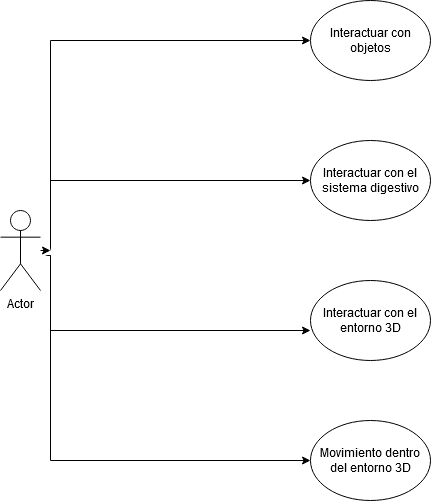
\includegraphics[width = .35\textwidth]{source/images/image36.png}
 		\captionof{figure}{\label{fig:im26}Diagrama de casos de uso del sistema}
	\end{center} 
\end{figure}

\section{Complicaciones del desarrollo sin metodología}
El proyecto comenzó su desarrollo sin tomar en cuenta la metodología de desarrollo Open UP, lo cual detonó en que el trabajo se viera mermado en cuanto a su documentación y desarrollo.\\
El desarrollo de un sistema mediante Open UP puede ser una herramienta poderosa para el desarrollo de software ya que dentro de ella se desarrollan micro incrementos en el desarrollo del software y además cumple con los principios del Manifiesto Ágil\cite{beck2001manifesto}.\\
La problemática surge cuando se intenta implementar en un proyecto de software diferente al cual usualmente se desarrolla, por ejemplo un Sistema de Calendarización de Trabajos terminales o un Generador de Páginas Web, difiere en cuanto a su desarrollo ya que se usan herramientas y elementos diferentes, tales como el desarrollo en el motor Unity ®, el diseño de los modelos 3D y el uso de elementos propietarios de Oculus ® dificultan la tarea de documentación y desarrollo bajo lineamientos por más ligeros que sean debido a la naturaleza del proyecto.\\
Es por eso que se buscó como alternativa una metodología que tome en cuenta las características inherentes de un software que su núcleo está arraigado a la realidad virtual haciéndolo un software multimedia.\\
Debido al cambio de enfoque de desarrollo de la metodología las tareas de reingeniería son suplementadas por más tiempo de desarrollo y refinamiento de los elementos anteriores a estos dentro del cronograma de actividades.\\


%\begin{figure}[H]
%	\begin{center}
% 		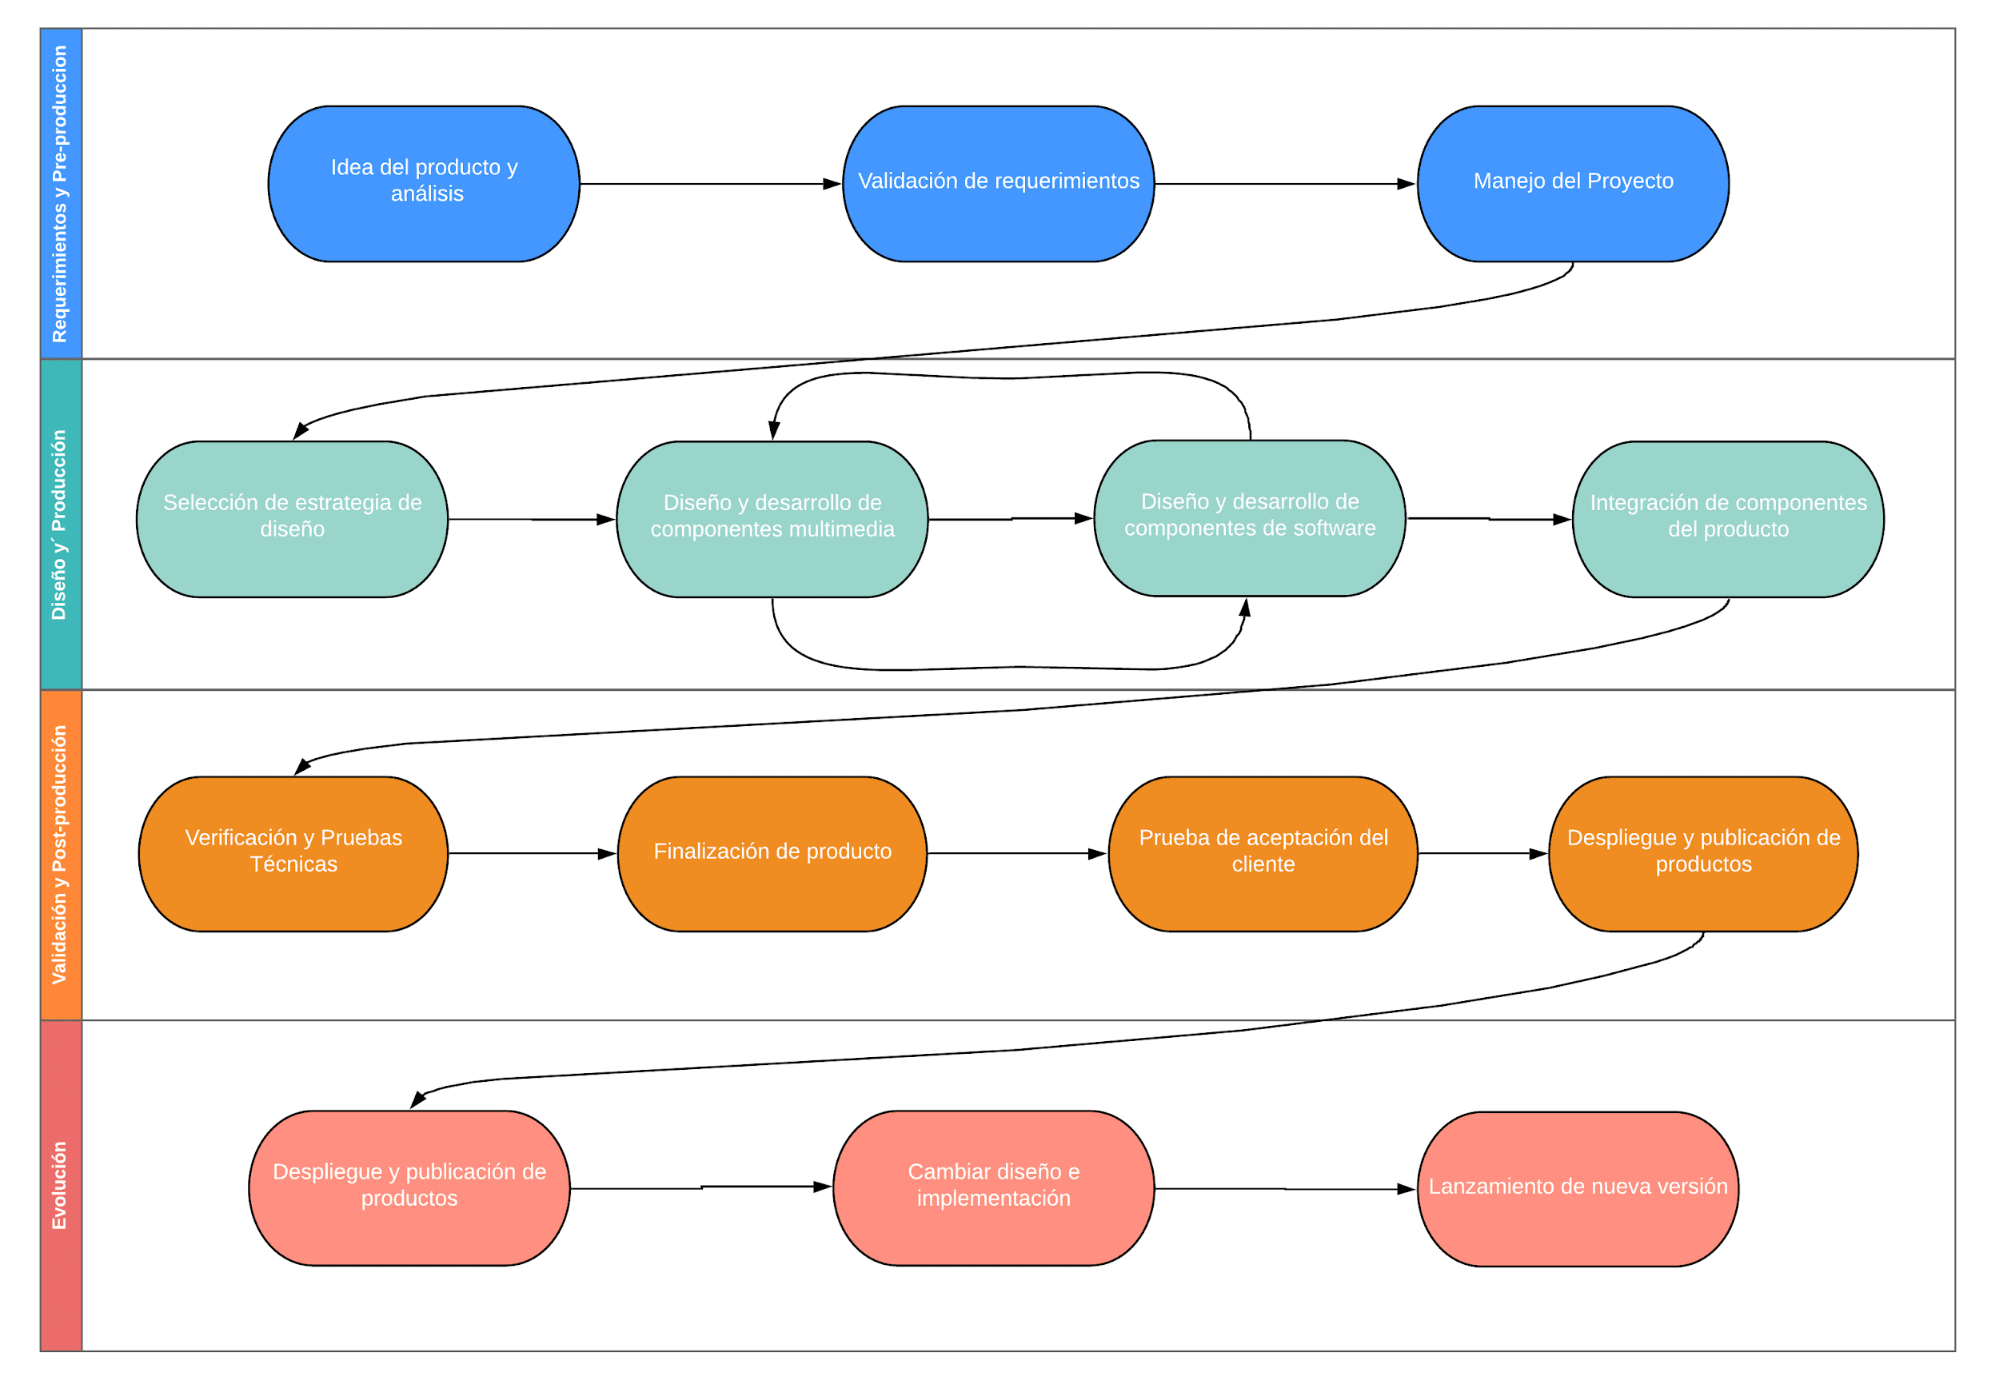
\includegraphics[width = 1\textwidth]{source/images/image50.png}
% 		\captionof{figure}{\label{fig:me2}Fases de la Metodología de ingeniería de software multimedia}
%	\end{center} 
%\end{figure}